\documentclass{llncs}

\usepackage{amsmath,amssymb,mathtools,nccmath}
\usepackage{paralist}
\usepackage{tabularx,booktabs}
\usepackage{multirow}
\usepackage{url}
\usepackage{tikz}
\usetikzlibrary{matrix,arrows,shapes,calc}
\usepackage%[colorlinks]
{hyperref}

\newcommand{\ite}[3]{\mathbf{if}\ #1\ \mathbf{then}\ #2\ \mathbf{else}\ #3\ \mathbf{fi}}
\newcommand{\power}[1]{2^{#1}}
\newcommand{\monus}{\;\,\mathtt{monus}\;\,}
\newcommand{\MA}{\mathcal{M}\!\!\mathcal{A}}
\newcommand{\AP}{\mathit{A\!P}}


\newcommand{\abs}{\ensuremath{\mathrm{abs}}}
\newcommand{\sign}{\ensuremath{\mathrm{sign}}}
\newcommand{\val}{\ensuremath{\mathit{val}}}

\newcommand{\eoe}{\hfill$\blacksquare$}

\begin{document}


\title{Modular SMT Encoding for Networks of  Nonlinear Hybrid Systems}
%\titlerunning{}

\author{Kyungmin Bae\inst{1} \and Soonho Kong\inst{2} \and Sicun Gao\inst{3} 
%\and Edmund M. Clarke\inst{1}
}
\institute{
SRI International
\and
Carnegie Mellon University
\and
Massachusetts Institute of Technology}

\maketitle
\begin{abstract}
Formal analysis problems of general hybrid systems, 
which involve
nonlinear %real functions and solutions of 
ordinary differential equations (ODEs), can be reduced to SMT problems over the real numbers. 
%
However, the standard SMT encoding experiences a new \emph{formula explosion problem}
for networks of nonlinear hybrid systems. % that makes their analysis practically infeasible.
Since continuous dynamics of tightly coupled components cannot be decomposed,
one cannot \emph{modularly} encode such systems using %standard 
SMT formulas over the real numbers.
%
In order to avoid this problem, we present a novel logical framework
to symbolically decompose ODE systems, which extends the standard theory over the real number by adding parameterized integration operators.
%
The experimental results show 
that our techniques greatly increase the performance of SMT-based analysis for networks of hybrid systems with %multiple modes and 
nonlinear ODEs.\end{abstract}



\section{Introduction}
\label{sec:intro}

%Formal analysis of hybrid systems is very difficult.
%Besides the difficulties from complex discrete controls,
%they typically involve continuous dynamics governed by ordinary differential equations (ODEs).
%%In order to cope with these challenges,
%%many important advances have been made by
%%various approaches. % including \cite{DBLP:journals/jlp/FranzleTE10,DBLP:conf/cav/FrehseGDCRLRGDM11,DBLP:journals/tac/AlthoffK14,DBLP:conf/hybrid/Frehse05,DBLP:conf/icons/HerdeEFT08,DBLP:conf/rtss/ChenAS12,DBLP:conf/aaai/CimattiMT12,platzer2008differential}.

Formal analysis problems of hybrid systems can be encoded as SMT formulas
over the real numbers.
In this approach, 
we can combine state-of-the-art SMT techniques 
with numerical algorithms for analyzing the continuous dynamics,
governed by ordinary differential equations (ODEs).
%
The satisfaction problems of these formulas are in general undecidable
for nonlinear hybrid systems.
%Since hybrid systems usually involve nonlinear real functions and (nonlinear) ODEs, 
But if we take into account robustness properties under numerical perturbations,
then they become \emph{decidable} up to any user-given precision $\delta >0$
using $\delta$-complete decision procedures \cite{delta-comp,sat-ode}.
This is very useful in practice, since sampling exact values of physical parameters is not possible in reality.

 
However, 
for \emph{networks of nonlinear hybrid systems},
their SMT-based  analysis is often unfeasible in practice.
One of the reasons is that
continuous connections between different components can be \emph{precisely} modeled
using \emph{coupled} systems of ODEs.
Consider, for example, three adjacent rooms: the temperature of one room 
continuously affects the temperature of the other rooms. 
The ODE systems for one room, modeling its behavior according to its control modes, 
also include the variables of the other rooms,
and  combinations of different ODE components give the behavior of the entire system.
%
Unlike the case of networks of restricted hybrid systems (e.g., linear hybrid systems),
a typical way to modularly encode parallel compositions
cannot be applied for such \emph{tightly coupled} nonlinear components,
because \emph{connected} variables evolve simultaneously over time.
% and thus ODE solving cannot be compositional. 


For this reason, existing SMT approaches can make use of only non-modular encodings 
for networks of nonlinear hybrid automata,
by explicitly enumerating all combinations of ODE components.
For a parallel composition $H_1 \parallel \cdots \parallel H_n$ of hybrid systems,
when each component $H_i$ includes $m_i$ ODE systems with respect to its control modes, % for $1 \leq i \leq n$,
by using the non-modular way to encode hybrid systems in SMT,
the size of the formula is $O(\prod_{i = 1}^n m_i)$.
This leads to the \emph{formula explosion problem}
that makes such SMT-based analysis practically infeasible.
%
The goal of this paper is to provide a logical framework for SMT
to effectively encode networks of nontrivial hybrid systems, 
involving nonlinear ODEs.

%We present a novel logical framework to provide an efficient SMT decision procedure for formulas produced by the new encoding (Section 4). Formulas given by the new encoding involve uninterpreted real functions and universal quantification. There is in general no effective decision procedure for checking the satisfaction of these formulas. But the full expressive power of extra function symbols and universal quantification is not necessary for hybrid automata. By extending the standard theory of real numbers with continuous functions, we show that SMT formulas for hybrid automata generated by the new encoding are equivalently expressed without uninterpreted real functions and universal quantification. Furthermore, their satisfaction problems in the new logical theory can be reduced to ones in the standard theory of real numbers at no cost.
%
%We present a new syntactic formulation to effectively encode formal analysis problems of networks of hybrid systems as SMT formulas in a modular way (Section 3). For a composition H1 ? ��� ? Hn of hybrid systems, when Hi has mi control modes for 1 ? i ? n, by using the standard way to encode analysis problems of hybrid systems in SMT, the formula contains k � ??i=1...n mi ODE literals for k-step bounded model checking. The size of the entire formula can be huge for networks of hybrid systems. We show that using uninterpreted real function symbols and universal quantification, we can construct a logically equivalent SMT formula with only k ODE literals, and thus the size of the resulting formula can be much smaller. This is practically very useful since a theory solver for nonlinear ODEs is computationally very expensive.

\paragraph{Our Contributions.}

We explain a new logical formulation to 
modularly encode networks of nonlinear hybrid systems
as SMT formulas.
We show that coupled systems of ODEs
can be decomposed by means of universal quantification over time,
by expressing continuous physical connections between components.
%in a modular way.
%(which the standard decomposition cannot correctly do).
The size of the SMT formula by the new modular encoding is $O(\sum_{i=1}^n m_i^2)$.

We then presents a novel logical framework for networks of nonlinear hybrid automata
that provides a simple decision procedure. %for the satisfiability of these formulas.
It extends the standard theory over the real number 
by adding parameterized integration operators,
 to logically decompose coupled ODE systems
without using\emph{universal quantification}.
The satisfaction problems in the new logical theory 
can be reduced to ones in the standard theory of the real numbers \emph{at no cost}.

We have implemented our technique within the \textsf{dReal} SMT solver~\cite{dReal},
and performed experiments on a number of nontrivial networked nonlinear hybrid systems. % (Section~\ref{sec:case-studies}).
The experimental results show that our techniques can dramatically increase 
the performance of SMT-based analysis for these networks of hybrid systems
that involve multiple control modes and nonlinear ODEs.
To the best of our knowledge, 
such networks of nonlinear hybrid systems
cannot be effectively analyzed by other existing SMT-based approaches for hybrid systems.


%Because of the difficulty of handling SMT formulas over the reals with nonlinear functions, SMT-solving-based verifi- cation is a fairly new direction for nonlinear hybrid systems. The research direction is initiated in [13], which uses con- straint solving algorithms for handling nonlinear reachability problems. Two main lines of work that explicitly formulate problems as SMT formulas are based on the HySAT/iSAT solver [14], [15] and the MathSAT solver [16], [17]. But neither efficient encodings of distributed hybrid systems nor inductive and compositional analysis has been investigated in existing work along these lines. 


\paragraph{Related Work.}

SMT-based verification is a fairly new direction for nonlinear hybrid systems,
because of the difficulty of handling SMT formulas over the real numbers with nonlinear functions.
The research direction is initiated in~\cite{DBLP:conf/hybrid/RatschanS05}, which uses constraint
solving algorithms for handling nonlinear reachability problems. 
Two main lines of work that explicitly 
formulate analysis problems as SMT formulas are based on the HySAT/iSAT
solver~\cite{DBLP:journals/fmsd/FranzleH07,DBLP:conf/atva/EggersFH08}
and the MathSAT solver~\cite{DBLP:conf/aaai/CimattiMT12,DBLP:conf/fmcad/CimattiMT12}.
%and the HyComp tool \cite{hycomp}.
But efficient encoding of networks of nonlinear hybrid systems has not been
investigated in existing work along these lines. 
%
Our techniques are orthogonal to 
reachable set computation techniques such as  
SpaceEX~\cite{DBLP:conf/cav/FrehseGDCRLRGDM11} 
and Flow*~\cite{DBLP:conf/cav/ChenAS13},
since they can also be used as ODE solvers for  SMT solving.



The \textsf{dReal} SMT solver \cite{dReal} can check the satisfiability of SMT formulas with nonlinear real functions and ODEs up to any precision $\delta >0$.
The \textsf{dReach} tool~\cite{dReach}
encodes reachability problems of nonlinear hybrid systems as SMT problems for \textsf{dReal}.
In order to deal with the formula explosion problem, 
\textsf{dReach} \emph{explicitly} enumerates
 all mode paths of a hybrid automaton
 by generating many small SMT formulas for these paths.
But the power of SMT techniques (such as DPLL($\mathcal{T}$) and CDCL)
cannot be fully exploited in this way.



The rest of the paper is organized as follows.
Section~\ref{sec:prelim} 
gives  some  background on hybrid automata and SMT.
Section~\ref{sec:effective-encoding} 
discusses modular encodings of networks of hybrid automata.
Section~\ref{sec:logic}
presents a new logical framework supporting the modular encodings of networks of \emph{nonlinear} hybrid automata.
Section~\ref{sec:case-studies} gives an overview of cast studies. % and experimental results.
%illustrates cast studies on various networks of hybrid systems.
Finally, Section~\ref{sec:concl} presents some conclusions.


\section{Preliminaries on Hybrid Automata and SMT}
\label{sec:prelim}

\paragraph{\bf Hybrid Automata.}

Hybrid systems are formally specified by \emph{hybrid automata} \cite{henzinger2000theory,lynch2003hybrid}.
%state machines with continuous variables.
%
Discrete states  are given by a set of modes $Q$.
Physical states are given by a finite set of real-valued variables $X = \{x_1, \ldots, x_l\}$,
where the domain of its values $\vec{v} = (v_1,\ldots,v_l)$ is denoted by $\val(X) =\mathbb{R}^l$.
%A combined state is %then 
%a pair $(q, \vec{v}) \in Q \times \val(X)$ of a mode $q$ and a vector $\vec{v} = (v_1,\ldots,v_l)$. % of real numbers.
%
For each mode $q \in Q$,
its invariant condition %$\mathit{inv}(q)$ 
defines all possible values of variables $X$, % in mode $q$,
and its flow condition %$\mathit{flow}(q)$ 
defines the continuous dynamics of $X$.
%
Discrete transitions between modes are given by jump conditions, identified with actions $a \in \Sigma$.
%
Let $\mathit{traj}(X)$ denote a set of \emph{trajectories} that describe the values of $X$ over time.
%(i.e., a trajectory of $\{x_1,\ldots,x_l\}$ of duration $t$ is a function $(f_1,\ldots,f_l) : [0,t] \to \val(X)$).

\begin{definition}
A \emph{hybrid automaton} is
$H = (X, Q, \Sigma, \mathit{init}, \mathit{inv}, \mathit{flow}, \mathit{jump})$ with:
%
\begin{inparaenum}[(i)]
	\item $X$ a set of real-valued variables; % = \{x_1, \ldots, x_l\}
	\item $Q$ a set of modes, 
	\item $\Sigma$ a set of actions;
	\item $\mathit{init} \subseteq Q \times \val(X)$ a set of initial states;
	\item $\mathit{inv} : Q \to \power{\val(X)}$ %assigns to each mode $q$ its invariant condition
	defining the set of all possible values of $X$ in mode $q$;
	\item $\mathit{flow} : Q \to \power{\mathit{traj}(X)}$ %assigns to each mode $q$ its flow condition
	defining the set of all trajectories of $X$ in mode $q$; and 	
	\item  $\mathit{jump} : (Q \times \val(X)) \times \Sigma \times (Q \times \val(X))$
	defining discrete transitions $(q, \vec{v}) \xrightarrow{a} (q', \vec{v'})$
	with action $a$.
\end{inparaenum}
\end{definition}

\noindent
The $\mathit{init}$, $\mathit{inv}$, and $\mathit{jump}$ conditions
are written as predicates over variables $X$:
for example, $\mathit{init}_q(\vec{x})$,
$\mathit{inv}_q(\vec{x})$,
and $\mathit{jump}_{q,a,q'}(\vec{x}, \vec{x'})$
for modes $q,q' \in Q$, action $a \in \Sigma$,
and vectors of variables $\vec{x}$ and $\vec{x'}$.
%
The  $\mathit{flow}$ condition
is written as a system of ordinary differential equations (ODEs)
of the form
$\dot{\vec{x}} = \mathit{flow}_q(\vec{x})$.
%where $\dot{x}_i$ denotes the first derivative $\frac{\mathrm{d}x_i}{\,\mathrm{d}t}$ of each variable $x_i$, $i = 1,\ldots,l$.


%\paragraph{\bf Parallel Composition of Hybrid Automata.}

Networks of hybrid systems can be formally specified by parallel compositions of hybrid automata.
For a parallel composition $H_1 \parallel H_2$, 
its mode is a pair $(q_1,q_2)$ % \in Q_1 \times Q_2
of $H_1$'s mode $q_1$ and $H_2$'s mode $q_2$,
and its physical state is given by the set of real-valued variables $X_1 \cup X_2$ from $H_1$ and $H_2$.
%
The continuous \emph{physical} interaction between $H_1$ and $H_2$ is modeled by using shared variables in $X_1 \cap X_2$,
and their discrete communication is modeled by using joint synchronous actions in $\Sigma_1 \cap \Sigma_2$.
%
For a physical state $\vec{v} \in \val(X_1\cup X_2)$,
let $\vec{v}\!\restriction_{X_i} \in \val(X_i)$
denote the projection of $\vec{v}$ onto variables $X_i$ for $i = 1,2$.
Similarly, for a trajectory $\vec{f} \in \mathit{traj}(X_1 \cup X_2)$,
let $\vec{f}\!\restriction_{X_i} \in \mathit{traj}(X_i)$
denote the restriction of $\vec{f}$ by %variables 
$X_i$. % for $i = 1,2$.

\begin{definition}
\label{def:comp}
The \emph{parallel composition}
of hybrid automata $H_1$ and $H_2$
%$H_i = (X_i, Q_i, \Sigma_i, \mathit{init}_i, \mathit{inv}_i, \mathit{flow}_i, \mathit{jump}_i)$
is the automaton $H_1 \parallel H_2 = 
(X_1 \cup X_2,\, Q_1 \times Q_2,\, \Sigma_1 \cup \Sigma_2,\, \mathit{init},\, \mathit{inv},\, \mathit{flow},\, \mathit{jump})$,
where:
%
\begin{itemize}
	\item $((q_1,q_2),\vec{v}) \in \mathit{init}$ iff $(q_1, \vec{v}\!\restriction_{X_1}) \in \mathit{init}_1$ and  $(q_2, \vec{v}\!\restriction_{X_2}) \in \mathit{init}_2$;
		
	\item $\vec{v} \in \mathit{inv}(q_1,q_2)$ iff $\vec{v}\!\restriction_{X_1} \in \mathit{inv}_1(q_1)$ and $\vec{v}\!\restriction_{X_2} \in \mathit{inv}_2(q_2)$;

	\item $\vec{f} \in \mathit{flow}(q_1,q_2)$ 
	iff $\vec{f}\!\restriction_{X_1} \in \mathit{flow}_1(q_1)$ and $\vec{f}\!\restriction_{X_2} \in \mathit{flow}_2(q_2)$; and
	 
	
	\item $((q_1,q_2), \vec{v}) \xrightarrow{a} ((q_1',q_2'), \vec{v'}) \in \mathit{jump}$ 
	iff 
%	both $H_1$ and $H_2$ synchronize their transitions with common action $a \in \Sigma_1 \cap \Sigma_2$; that is,
	for each $i = 1,2$:
	\begin{inparaenum}[(i)]
		\item if $a \in \Sigma_i$, then $(q_i, \vec{v}\!\restriction_{X_i}) \xrightarrow{a} (q_i', \vec{v'}\!\restriction_{X_i}) \in \mathit{jump}_i$, and 
		\item if $a \notin \Sigma_i$, then no transition of $H_i$ is taken  (that is, $(q_i,\vec{v}\!\restriction_{X_i}) = (q_i',\vec{v'}\!\restriction_{X_i})$).
	\end{inparaenum}
%	\[
%	\begin{cases}
%	(q_i, \vec{v}\!\restriction_{X_i}) \xrightarrow{a} (q_i', \vec{v'}\!\restriction_{X_i}) \in \mathit{jump}_i 
%	& \mbox{if}\;\;a \in \Sigma_i
%	\\
%	(q_i,\vec{v}\!\restriction_{X_i}) = (q_i',\vec{v'}\!\restriction_{X_i})
%%	\;\wedge\; (q_i = q_i') \;\wedge\; (\vec{v}\!\restriction_{X_i} = \vec{v'}\!\restriction_{X_i})
%	& \mbox{if}\;\;a \notin \Sigma_i.
%	\end{cases}
%	\]
\end{itemize}
\end{definition}


\begin{example}[Physically Networked Thermostat Controllers]
\label{ex:net-thermo}
Consider 
a network of classical thermostat hybrid automata 
(the specification of a single hybrid automaton is adapted from \cite{henzinger2000theory}). 
A number of rooms are interconnected by open doors,
and the temperature of each room is separately controlled by each thermostat
that turns its heater on and off,
as depicted in Figure~\ref{fig:adj-rooms}.

The temperature $x_i$  of room $i$ depends on
the heater's mode $q_i \in \{m_\mathtt{on}, m_\mathtt{off}\}$  and the temperatures of the adjacent rooms.
The value of $x_i$
changes according to the ODEs,
where $A_i \subseteq \mathbb{N}$ denotes the set of its adjacent rooms:
\[
\dot{x_i} =
\begin{cases}
K_i \big(h_i - (x_i \cdot (1- \sum_{j \in A_i} k_{i,j})  + \sum_{j \in A_i} x_j k_{i,j}  )\big)
& \mbox{if}\;\; q_i = m_\mathtt{on},
\\
- K_i \big(x_i \cdot (1- \sum_{j \in A_i} k_{i,j})  + \sum_{j \in A_i} x_j k_{i,j}  \big)
& \mbox{if}\;\; q_i = m_\mathtt{off}.
\end{cases}
\]
The constants $K_i, h_i, k_{i,j} \in \mathbb{R}$ depend on
the size of room $i$,  the heater's power, and the size of the open door between rooms $i$ and $j$, respectively.
Notice that the ODEs for room $i$ include variables $x_j$ for adjacent rooms $j \in A_i$.

%The physical interaction between adjacent rooms is modeled using the ODEs.

Every thermostat controller synchronously performs its discrete transitions with common action $a$.
For each second,  the heater is turned on if $x_i \leq T_{\min}^i$, and turned off if $x_i > T_{\max}^i$.
To keep track of each one-second period,
every automaton has a \emph{shared} timer variable $\tau$ 
with the flow condition $\dot{\tau} = 1$.


The hybrid automaton $H_i = (X_i, Q_i, \Sigma_i, \mathit{init}_i, \mathit{inv}_i, \mathit{flow}_i, \mathit{jump}_i)$ %for room~$i$
is defined in an expected way.
 For example:
\begin{inparaenum}[(i)]
	\item $X_1 = \{x_1, x_2, \tau\}$,
	\item $Q_1 = \{q_\mathtt{on}, q_\mathtt{off}\}$,
	\item $\Sigma_1 = \{a\}$,
	\item $\mathit{init}_1 = \{(q_\mathtt{off}, v_1, v_2, \tau) \mid T_{\min}^i < v_1, v_2 < T_{\max}^i, \tau = 0\}$,
	\item $\mathit{inv}_1(q) = \{(v_1, v_2, \tau) \mid 0 \leq \tau \leq 1\}$,
	\item $\mathit{flow}_1(q)$ given by the ODEs for $\dot{x_1}$ and $\dot{\tau}$,
	\item $(q, v_1,v_2,1) \xrightarrow{a} (q', v_1,v_2,0) \in \mathit{jump}$
	iff 
	$(x_i \leq T_{\min}^i \rightarrow q' = q_\mathtt{on})$,
	$(x_i > T_{\max}^i \rightarrow q' = q_\mathtt{off})$, and
	$(T_{\min}^i < x_i \leq T_{\max}^i \rightarrow q' = q)$.
\end{inparaenum}
%Notice that $X_0$ also includes the temperature $x_1$ of room $1$,
%since room~$1$ is adjacent to room $0$
%and therefore the flow condition of $H_0$ depends on $x_1$ as well as $x_0$.
\eoe
\end{example}


\begin{figure}[t]
\centering
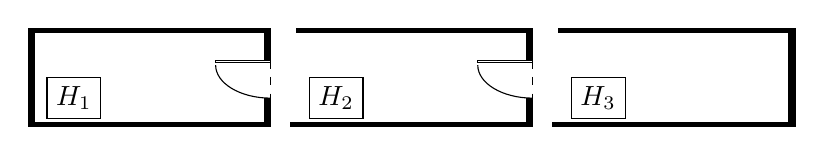
\begin{tikzpicture}[yscale=0.60] %baseline=(current bounding box.north)
%room1
\begin{scope}
\filldraw (0,-0.6) rectangle  + (-0.08,0.6)
	(0,0) rectangle  + (-3,0.08)
	(-3.08,-2.0) rectangle  + (3,0.08)
	(-3,0.08) rectangle  + (-0.08,-2.0)
	(0,-2.0) rectangle  + (-0.08,0.6);
	\draw[dashed] (0,-0.6) -- (0,-2);
	\draw (0,-0.6) rectangle +(-0.7,-0.05);
	\draw (-0.7,-0.7) arc (180:270:0.7);
	\path (-2.5,-1.4) node[draw] { $H_1$};
\end{scope}
%room2
\begin{scope}[xshift=22ex]
\filldraw (0,-0.6) rectangle  + (-0.08,0.6)
	(0,0) rectangle  + (-3,0.08)
	(-3.08,-2.0) rectangle  + (3,0.08)
	(0,-2.0) rectangle  + (-0.08,0.6);
	\draw[dashed] (0,-0.6) -- (0,-2);
	\draw (0,-0.6) rectangle +(-0.7,-0.05);
	\draw (-0.7,-0.7) arc (180:270:0.7);
	\path (-2.5,-1.4) node[draw] { $H_2$};
\end{scope}
%room3
\begin{scope}[xshift=44ex]
\filldraw (0,-2.0) rectangle  + (-0.08,2.0)
	(0,0) rectangle  + (-3,0.08)
	(-3.08,-2.0) rectangle  + (3,0.08);
	\path (-2.5,-1.4) node[draw] { $H_3$};
\end{scope}
\end{tikzpicture}
\caption{Three interconnected rooms by open doors.
} \label{fig:adj-rooms}
\end{figure}





\paragraph{\bf Standard Encoding of Hybrid Systems in SMT.}

An SMT (satisfiability modulo theories) problem is to check the satisfiability of first-order formulas 
with respect to certain decidable logical theories.
Formal analysis of hybrid systems can be reduced to the satisfiability of SMT formulas
over the real numbers, along with computable real functions, including polynomials, %exponentiation, 
trigonometric functions, and solutions of Lipschitz-continuous ODEs.
The satisfiability of such formulas is generally undecidable for nonlinear real functions,
but the satisfiability \emph{up to a given precision $\delta >0$}
is decidable for nonlinear real functions 
using $\delta$-complete decision procedures \cite{delta-comp,sat-ode}, 
implemented in the \textsf{dReal} SMT solver \cite{dReal}.



\begin{definition}
Given a finite set $\mathcal{F}$ of computable real functions
(real constants given by $0$-ary functions),
$\mathcal{L}_\mathcal{F} = (\mathcal{F}, >)$ denotes the first-order signature over the real numbers
with the real functions in $\mathcal{F}$,
and $\mathbb{R}_\mathcal{F} = (\mathbb{R}, \mathcal{F}^\mathbb{R}, >^\mathbb{R})$
is the standard structure for the theory of the real numbers.
\end{definition}

The behavior of a hybrid automaton 
$H = (X, Q, \Sigma, \mathit{init}, \mathit{inv}, \mathit{flow}, \mathit{jump})$
can be encoded as $\mathcal{L}_\mathcal{F}$-formulas.
As mentioned earlier, discrete jumps $(q, \vec{v}) \xrightarrow{a} (q', \vec{v'})$
are expressed as $\mathcal{L}_\mathcal{F}$-predicates $\mathit{jump}_{q,a,q'}(\vec{v}, \vec{v'})$.
The continuous change of $X$'s values in mode $q$ 
from $\vec{v^0}$ to $\vec{v^t}$ for duration $t$
according to the ODE system $\dot{\vec{x}} = \mathit{flow}_q(\vec{x})$
is expressed as the $\mathcal{L}_\mathcal{F}$-formula
\[
\mathit{flow}_q(\vec{v^0},\vec{v^t},t) 
\;\;\equiv\;\;
\Big(
\vec{v^t} = \vec{v^0} + \int_{0}^t \mathit{flow}_q(\vec{x}) \,\mathrm{d}t
\Big)
\]
where the integral $\int_{0}^t \mathit{flow}_q(\vec{x}) \,\mathrm{d}t$ is considered as a real function over time~$t$. % in $\mathcal{L}_\mathcal{F}$.
To state that the invariant condition holds for any continuous trajectories of $X$ from $\vec{v^0}$ for duration $t$ in mode $q$, 
we write the $\mathcal{L}_\mathcal{F}$-formula:%
\footnote{\textsf{dReal} can handle such universally quantified formulas over the time variable $u$.}
\[
\mathit{inv}_q(\vec{v^0},t) 
\;\;\equiv\;\;
\forall u \in [0,t], \forall \vec{x^u}.\;\;  %\in \val(X)
\mathit{flow}_q(\vec{v^0},\vec{x^u},u) \,\to\,
\mathit{inv}_q(\vec{x^u})
\]


\begin{example}[Isolated Single Thermostat]
\label{ex:isolated}
Consider a hybrid automaton for one room in Example~\ref{ex:net-thermo},
but all its doors are closed, and thus the ODEs only depend on 
the room's temperature $x$. The flow condition is expressed as the $\mathcal{L}_\mathcal{F}$-formulas:
\begin{align*}
\mathit{flow}_\mathtt{on}([x^0,\tau^0],[x^t,\tau^t],t) 
\;\equiv\;&
\textstyle
\big(
[x^t,\tau^t] = [x^0,\tau^0] + \int_{0}^t [K (h - x(t)), 1] \,\mathrm{d}t
\big)
\\
\mathit{flow}_\mathtt{off}([x^0,\tau^0],[x^t,\tau^t],t)
\;\equiv\;&
\textstyle
\big(
[x^t,\tau^t] = [x^0,\tau^0] + \int_{0}^t [- K x(t),1] \,\mathrm{d}t
\big)
\end{align*}
%
For the jump condition, % the $\mathcal{L}_\mathcal{F}$-formula:
$\mathit{jump}_{q,a,q'}([x,\tau], [x', \tau'])
\;\equiv\;
(x \leq T_{\min} \rightarrow q' = q_\mathtt{on}) 
\,\wedge\, 
(x > T_{\max} \rightarrow q' = q_\mathtt{off})
\,\wedge\, 
(T_{\min} < x \leq T_{\max} \rightarrow q' = q)
\,\wedge\, 
(\tau = 1  \wedge  \tau'  = 0)$.
\eoe
\end{example}


The bounded reachability problem of a hybrid automaton $H$ up to its $k$-th step 
can be encoded as the following $\mathcal{L}_\mathcal{F}$-formula
whose satisfiable assignments give counterexamples of length $k$,
where
$t_{\max} > 0$ is a maximal duration of single modes, and
$\mathit{safe}(\vec{x})$ is a predicate to denote a safe region of $X$:
%
\begin{equation}
\label{eq:bounded-standard}
\begin{alignedat}{2}
\exists m_0,\ldots,m_k,\;
\vec{x_0^0}, \ldots, \vec{x_k^0}, \vec{x_0^t}, \ldots, \vec{x_k^t},\;  %\in \val(X)
\exists t_0, \ldots, t_k \in [0,t_{\max}].
\\
\begin{alignedat}{2}
\bigvee_{q \in Q}
\left[
m_0 = q 
\;\wedge\;
\mathit{init}_q(\vec{x^0_0}) 
\;\wedge\;
\mathit{flow}_q(\vec{x_0^0}, \vec{x_0^t}, t_0)
\;\wedge\;
\mathit{inv}_q(\vec{x_0^0}, t_0)
\right]
\\
\wedge\;
\bigwedge_{i = 1}^k\,
\bigvee_{\substack{q, r \in Q\\ a \in \Sigma}}
\left[
\begin{aligned}
m_{i-1} = q
\;\wedge\;
m_i = r
\;\wedge\;
\mathit{jump}_{q,a,r}(\vec{x_{i-1}^t},\vec{x_{i}^0})
\\
\wedge\;
\mathit{flow}_{r}(\vec{x_i^0}, \vec{x_i^t}, t_i)
\;\wedge\;
\mathit{inv}_{r}(\vec{x_i^0}, t_i)
\end{aligned}
\right]
\;\wedge\;
\neg \mathit{safe}(\vec{x_k^t})
\end{alignedat}
\end{alignedat}
\end{equation}
%
Each $i$-th step is in mode $m_i$,
has duration $t_i$,
begins with $\vec{x_i^0}$, and ends with $\vec{x_i^t}$.
%
In the initial step,
for \emph{some} mode  $q$,
the $\mathit{init}$ condition %of mode $q$  
holds on  $\vec{x_0^0}$,
$X$'s values changes 
from $\vec{x_0^0}$ to $\vec{x_0^t}$ during $t_0$
according to the $\mathit{flow}$ condition, %of mode $q$ 
and the $\mathit{inv}$ condition %of mode $q$ 
holds in the meantime. % for these trajectories.
%
The $i$-th intermediate step is reached 
iff for \emph{some} modes $q, r \in Q$, % and action $a \in \Sigma$, 
a discrete jump $q \xrightarrow{a} r$ happens from 
the final values $\vec{x_{i-1}^t}$ of the $(i-1)$-th step
to the starting values $\vec{x_{i}^0}$, % of the $i$-th step,
and then $X$'s values changes 
 from $\vec{x_{i}^0}$ to $\vec{x_{i}^t}$ during $t_i$
according to the $\mathit{flow}$ and $\mathit{inv}$ conditions of mode $r$.



\section{$\mathcal{L}_\mathcal{F}$-Encoding for Networks of Hybrid Automata}
\label{sec:effective-encoding}

In principle, 
a network of hybrid automata can always be encoded as 
$\mathcal{L}_\mathcal{F}$-formulas using Formula~(\ref{eq:bounded-standard})
by explicitly using their parallel composition.
%
However, the size of the resulting formula can be huge.
For a network of hybrid automata $H_1, \ldots, H_n$,
if each automaton $H_i$ has $m_i$ modes, % for $i = 1,\ldots,n$,
then a parallel composition $H_1 \parallel \ldots \parallel H_n$
has $\prod_{i = 1}^n m_i$ modes.
For $k$-step bounded reachability,
the size of the formula by Encoding~(\ref{eq:bounded-standard}) is 
$O(k \cdot \prod_{i = 1}^n m_i)$.

To avoid this \emph{formula explosion problem},
we need to encode networks of hybrid automata in a modular way.
%This section discusses modular encodings of networks of \emph{nonlinear} hybrid automata in the standard logic $\mathcal{L}_\mathcal{F}$.
For networks of \emph{nonlinear} hybrid automata,
%We argue that 
a main difficulty comes from the physical connections between %the ODEs of 
\emph{tightly coupled} components. %physically
%different components in networks of \emph{physically coupled} nonlinear hybrid automata.
%the flow condition of one hybrid automaton is continuously synchronized with the flow condition of others
%(e.g.,  Example~\ref{ex:net-thermo}).
%
%We explain why 
The standard decomposition technique, 
that has been widely used for \emph{restricted} hybrid automata, 
does not work %in general 
for  physically coupled nonlinear hybrid automata.
We present a new $\mathcal{L}_\mathcal{F}$-formulation to modularly encode  such networks of nonlinear hybrid automata 
in a logically correct way. 
%
%A new technique to address this challenge is shown in Section~\ref{sec:logic}.


\paragraph{\bf Standard Decomposition.}

A standard way to modularly encode a parallel composition $H_1 \parallel \cdots \parallel H_n$ is to take into account synchronization conditions.
%Consider a parallel composition $H_1 \parallel \cdots \parallel H_n$.
For each %hybrid automaton 
$H_j$,
we extend the meaning of the jump predicate $\mathit{jump}^j$ 
for general actions $\Sigma_1 \cup \cdots \cup \Sigma_n$
according to Definition~\ref{def:comp}:
$\mathit{jump}^j_{q_j,a,q_j'}(\vec{x_j}, \vec{x_j'}) = \mathit{jump}^j_{q_j,a,q_j'}(\vec{x_j}, \vec{x_j'})$
if $a \in \Sigma_j$, 
and $q_j = q_j' \;\wedge\; \vec{x_j'} = \vec{x_j}$ if $a \notin \Sigma_j$.
%\[
%\mathit{jump}^j_{q_j,a,q_j'}(\vec{x_j}, \vec{x_j'})
%\;\equiv\;
%\begin{cases}
%	\mathit{jump}^j_{q_j,a,q_j'}(\vec{x_j}, \vec{x_j'}) 
%	& \mbox{if}\;\;a \in \Sigma_j
%	\\
%	q_j = q_j' \;\wedge\; \vec{x_j'} = \vec{x_j}
%	& \mbox{if}\;\;a \notin \Sigma_j.
%\end{cases}
%\]

Assuming that \emph{the flow condition of each %hybrid 
automaton can be fully encoded as $\mathcal{L}_\mathcal{F}$-formulas},
a $k$-step bounded reachability problem of $H_1 \parallel \cdots \parallel H_n$
can then be  encoded as the following $\mathcal{L}_\mathcal{F}$-formula of size $O(k \cdot \sum_{j = 1}^n m_j^2)$:
%
\begin{equation}
\label{eq:bounded-standard-comp}
\begin{alignedat}{2}
\exists \{m_0^j,\ldots,m_k^j,\;
	\vec{{x_j}_0^0}, \ldots, \vec{{x_j}_k^0}, \vec{{x_j}_0^t}, \ldots, \vec{{x_j}_k^t}\}_{j=1}^n,\;
\exists t_0, \ldots, t_k \in [0,t_{\max}].
\\
\begin{alignedat}{2}
\bigwedge_{j=1}^n
\smashoperator[r]{\bigvee_{q_j \in Q_j}}
\left[
m_0^j = q_j 
\;\wedge\;
\mathit{init}^j_{q_j}(\vec{{x_j}^0_0}) 
\;\wedge\;
\mathit{flow}^j_{q_j}(\vec{{x_j}_0^0}, \vec{{x_j}_0^t}, t_0)
\;\wedge\;
\mathit{inv}^j_{q_j}(\vec{{x_j}_0^0}, t_0)
\right]
\\
\wedge\;
\bigwedge_{j=1}^n
\bigwedge_{i = 1}^k\quad
\bigvee_{\mathclap{\substack{q_j, r_j \in Q\\ a \in \bigcup_{l=1}^n \Sigma_l}}}\;\;\,
\left[
\begin{aligned}
(m_{i-1}^j,m_i^j) = (q_j, r_j)
\;\wedge\;
\mathit{jump}^j_{q_j,a,r_j}(\vec{{x_j}_{i-1}^t},\vec{{x_j}_{i}^0})
\\
\wedge\;
\mathit{flow}^j_{r_j}(\vec{{x_j}_i^0}, \vec{{x_j}_i^t}, t_i)
\;\wedge\;
\mathit{inv}^j_{r_j}(\vec{{x_j}_i^0}, t_i)
\end{aligned}
\right]
\\[-1ex]
\wedge\;
\neg 
\bigwedge_{j=1}^n\,
\mathit{safe}(\vec{{x_j}_k^t})
\end{alignedat}
\end{alignedat}
\end{equation}
%
The behavior of each hybrid automaton is separately encoded using Formula~(\ref{eq:bounded-standard}).
Whenever a discrete jump is taken by one hybrid automaton, all components synchronize on it using synchronization conditions.
Flow conditions are assumed to be synchronized  upon mode changes using mode variables.


The standard decomposition technique can be applied to various classes of restricted hybrid automata, 
such as linear hybrid automata and piecewise affine hybrid automata.
The flow conditions of a single hybrid automaton in such classes are independently expressed 
by real functions of specified ``solved'' forms,
and therefore they can be fully encoded as $\mathcal{L}_\mathcal{F}$-formulas.
%Many hybrid systems considered for formal verification in literature are belong to these classes.

But what about a very generic class of hybrid automata involving nonlinear ordinary differential equations (ODEs)?
In this cases, 
for a network of hybrid automata,
the ODEs for one hybrid automaton $H_i$ can be physically coupled with the ODEs for other automata;
that is, the derivatives of some ODE variables are \emph{not} specified in $H_i$, but in other hybrid automata.
Therefore, the standard decomposition technique cannot be directly applied,
%for such networks of hybrid systems,
since the ODEs for a single hybrid automaton cannot be (even numerically) evaluated.
%


\begin{example}
\label{ex:three-case}
Consider the network of three thermostat controllers in Example~\ref{ex:net-thermo}.
The hybrid automaton $H_1$ for room~$1$, adjacent to rooms $2$,
has the variable set $X_1 = \{x_1, x_2, \tau\}$,
and involves the ODEs %for its flow conditions
$\dot{x_1} = 7 - (0.9 x_1  + 0.1 x_2  )$ for $q_1 = m_\mathtt{on}$,
and 
$\dot{x_1} = - (0.9 x_1 + 0.1 x_2 )$ for $q_1 = m_\mathtt{off}$,
(where $K_1 = 1, h_1 = 7, k_{1,2} = 0.1$).
%\[
%\dot{x_1} =
%\begin{cases}
%7 - (0.9 x_1  + 0.1 x_2)
%& \mbox{if}\;\; q_1 = m_\mathtt{on},
%\\
%-  (0.9 x_1 + 0.1 x_2 )
%& \mbox{if}\;\; q_1 = m_\mathtt{off},
%\end{cases}
%\]
The predicates $\mathit{flow}^1_\mathtt{on}$ 
and $\mathit{flow}^1_\mathtt{off}$ for the flow conditions are then expressed by:
%
\begin{align*}
\mathit{flow}^1_\mathtt{on}(
\left[
\begin{medsize}
\begin{array}{c}
x_1^0\\
x_2^0\\
\tau^0
\end{array}
\end{medsize}
\right],
\left[
\begin{medsize}
\begin{array}{c}
x_1^t\\
x_2^t\\
\tau^t
\end{array}
\end{medsize}
\right],
t)
\;\equiv\;&
\left[
\begin{medsize}
\begin{array}{c}
x_1^t\\
x_2^t\\
\tau^t
\end{array}
\end{medsize}
\right]
= 
\left[
\begin{medsize}
\begin{array}{c}
x_1^0\\
x_2^0\\
\tau^0
\end{array}
\end{medsize}
\right]
+ 
\int_{0}^t 
\left[
\begin{medsize}
\begin{array}{c}
7 - (0.9 x_1(t)  + 0.1 x_2(t))\\
\dot{x_2}(t)\\
1
\end{array}
\end{medsize}
\right]
\mathrm{d}t
\\
%%%%%%
\mathit{flow}^1_\mathtt{off}(
\left[
\begin{medsize}
\begin{array}{c}
x_1^0\\
x_2^0\\
\tau^0
\end{array}
\end{medsize}
\right],
\left[
\begin{medsize}
\begin{array}{c}
x_1^t\\
x_2^t\\
\tau^t
\end{array}
\end{medsize}
\right],
t)
\;\equiv\;&
\left[
\begin{medsize}
\begin{array}{c}
x_1^t\\
x_2^t\\
\tau^t
\end{array}
\end{medsize}
\right]
= 
\left[
\begin{medsize}
\begin{array}{c}
x_1^0\\
x_2^0\\
\tau^0
\end{array}
\end{medsize}
\right]
+ 
\int_{0}^t 
\left[
\begin{medsize}
\begin{array}{c}
- (0.9 x_1(t) + 0.1 x_2(t) )\\
\dot{x_2}(t)\\
1
\end{array}
\end{medsize}
\right]
\mathrm{d}t
\end{align*}
%
These predicates contain the \emph{uninterpreted function} $\dot{x_2}$ in the integral terms 
whose interpretation is given by the other automata $H_2$ and $H_3$
(this is different from the isolated case in Example~\ref{ex:isolated} where $H_1$ only include $x_1$ and $\tau$).
It is \emph{not} possible to evaluate the integration of the ODEs with the uninterpreted function $\dot{x_2}$ by themselves.
%
In particular, 
the flow predicates have no meaning in %the standard theory 
$\mathbb{R}_\mathcal{F}$.
%since $\dot{x_2}$ may not be a computable real function.
\eoe
\end{example}


The point is that to modularly encode networks of \emph{tightly coupled} nonlinear hybrid automata,
we need %an effective way 
to  express the physical correlations between different components.
%which is lack in Formula~(\ref{eq:bounded-standard-comp}).
Since all variables in a system of ODEs evolve simultaneously over continuous time,
naive decoupling as in Formula~(\ref{eq:bounded-standard-comp}) does not work. % in general.
%We can approximate the continuous behavior of other components 
%(e.g., by setting some constant bounds for $\dot{x_2}$), 
%This technique is widely used for restricted models (e.g., linear hybrid automata),
%but this technique is not precise enough for analyzing nonlinear hybrid systems 
%using $\delta$-complete SMT.
%Of course,
By explicitly constructing parallel compositions,
we can still use Formula~(\ref{eq:bounded-standard}),
but at the cost of the formula explosion problem.
It is %indeed 
very difficult to modularly encode such physical correlations 
as $\mathcal{L}_\mathcal{F}$-formulas by using \emph{only concrete functions},
since each variable may have many solution functions for different combinations of ODEs.
In Example~\ref{ex:three-case}, 
$x_1$ depends on $x_2$, which again depends on $x_3$,
and therefore solutions functions of $x_1$ has $2^3 = 8$ different solved forms.


\paragraph{\bf Logically Correct Flow Decomposition.}

For networks of general nonlinear hybrid automata, 
the standard decomposition technique using Formula~(\ref{eq:bounded-standard-comp})
is semantically incorrect as previously stated,
since flow predicates may include ``undefined'' functions
 (e.g., see Example~\ref{ex:three-case}).
%
Adding extra terms to Formula~(\ref{eq:bounded-standard-comp})
for defining the semantics of such uninterpreted functions
(that is, the continuous interconnections between different components),
we can obtain a logically correct $\mathcal{L}_\mathcal{F}$-formula 
for networks of hybrid automata.
%
Since ODE variables may have many solved forms for different combinations of ODEs,
we consider \emph{parameterized flow predicates} to avoid the formula explosion problem.
%
The idea presented here is also carried over into 
a new logical framework in Section~\ref{sec:logic}.


We decompose each flow predicate
into a conjunction of several formulas
according to its structure. 
Consider a flow predicate 
for an $l$-dimensional ODEs
$\mathit{flow}_q(\vec{x^0},\vec{x^t},t)
\,\equiv\,
(\vec{x^t} = \vec{x^0} + \int_{0}^t \mathit{flow}_q(\vec{x})\,\mathrm{d}t)$.
Mathematically,
a variable $x$ in $\mathit{flow}(\vec{x})$ 
is a unary real function $\mathbb{R} \to \mathbb{R}$ over time,
and thus
$\mathit{flow}_q(\vec{x})$ can also be considered as a unary function
$\mathbb{R} \to \mathbb{R}^l$.
%
Therefore,
using extra function symbols $\dot{x_1}, \ldots, \dot{x_l}: \mathbb{R} \to \mathbb{R}$
to denote the derivatives of $\vec{x} = (x_1,\ldots,x_l)$,
the flow predicate can be rewritten as the logically equivalent conjunction: 
\[
\vec{x^t} = \vec{x^0} + \int_{0}^t [\dot{x_1}(t), \ldots, \dot{x_l}(t)]  \,\mathrm{d}t
\;\wedge\;
\forall u \in [0,t].\; [\dot{x_1}(u), \ldots, \dot{x_l}(u)] = \mathit{flow}(\vec{x})(u).
\]
The invariant condition \emph{with respect to an arbitrary flow $\vec{x}$} 
is similarly expressed as $\mathcal{L}_\mathcal{F}$-formulas using extra function symbols $\dot{\vec{x}} = (\dot{x_1}, \ldots, \dot{x_l})$.
The formula 
$\mathit{inv}(m,\vec{x})
\,\equiv\,
\bigwedge_{q \in Q} (m = q) \to \mathit{inv}_q(\vec{x})$
uniformly expresses invariant predicates
in such a way that $\mathit{inv}(q,\vec{x}) \equiv \mathit{inv}_q(\vec{x})$ for mode $q$.
Then, let us define:
\begin{align*}
\mathit{flow}_{\dot{\vec{x}}}(\vec{x^0},\vec{x^t},t) 
\;\;\equiv\;\;&
\vec{x^t} = \vec{x^0} + \int_{0}^t \dot{\vec{x}}(t)  \,\mathrm{d}t,
\\
\mathit{inv}_{\dot{\vec{x}}}(m,\vec{x^0},t) 
\;\;\equiv\;\;&
\forall u \in [0,t], \forall \vec{x^u}.\;\; %\in \val(X)
\mathit{flow}_{\dot{\vec{x}}}(\vec{x^0},\vec{x^u},u)  \,\to\,
\mathit{inv}(m,\vec{x^u}).
\end{align*}


\begin{example}
\label{ex:three-case2}
Consider the flow predicates $\mathit{flow}^1_\mathtt{on}$ and $\mathit{flow}^1_\mathtt{off}$
in Example~\ref{ex:three-case}. % for the network of three thermostat controllers.
The parameterized flow predicate 
$\mathit{flow}^1_{(\dot{x_1},\dot{x_2},\dot{\tau})}([x_1^0,x_2^0,\tau^0],[x_1^t,x_2^t,\tau^t],t)$
using extra function symbols $\dot{\vec{x_1}} = (\dot{x_1},\dot{x_2},\dot{\tau})$
is defined by the formula:
\[
[x_1^t,x_2^t,\tau^t]
=
[x_1^0,x_2^0,\tau^0]
+
\int_{0}^t [\dot{x_1}(t),\dot{x_2}(t),\dot{\tau}(t)] \,\mathrm{d}t.
\]
For $\vec{x_1^0} = (x_1^0,x_2^0,\tau^0)$ and $\vec{x_1^t} = (x_1^t,x_2^t,\tau^t)$,
the flow predicates
$\mathit{flow}^1_\mathtt{on}(\vec{x_1^0},\vec{x_1^t},t)$
and 
$\mathit{flow}^1_\mathtt{off}(\vec{x_1^0},\vec{x_1^t},t)$,
respectively,
are equivalently rewritten to the formulas:
%
\begin{align*}
\mathit{flow}^1_{\dot{\vec{x_1}}}(\vec{x_1^0},\vec{x_1^t},t)
\;\wedge\;&
\forall u \in [0,t].\; 
\dot{\tau}(u) = 1
\;\wedge\;
\dot{x_1}(u) = 7 - (0.9 x_1(u)  + 0.1 x_2(u)) 
\\
\mathit{flow}^1_{\dot{\vec{x_1}}}(\vec{x_1^0},\vec{x_1^t},t)
\;\wedge\;&
\forall u \in [0,t].\; 
\dot{\tau}(u) = 1
\;\wedge\; 
\dot{x_1}(u) = -  (0.9 x_1(t) + 0.1 x_2(t) ) 
\end{align*}
%
The universally quantified subformulas
\emph{assign} to the function symbols $\dot{x_1}$ and $\dot{\tau}$
their logical interpretation.
Notice that the interpretation of $\dot{x_2}$
can easily be assigned in a similar way by another hybrid automaton.
\eoe
\end{example}


Recall that the continuous behavior of a hybrid automaton
in mode $q$ from $\vec{x^0}$ to $\vec{x^t}$ for duration $t$
is expressed as the formula
$\mathit{flow}_q(\vec{x^0}, \vec{x^t}, t) \;\wedge\; \mathit{inv}_q(\vec{x^0}, t)$,
which can also be decomposed into the logically equivalent conjunction.

\begin{lemma}
\label{lem:cont-equiv}
The following $\mathcal{L}_\mathcal{F}$-formulas are logically equivalent to each other:
\begin{alignat*}{2}
	&\mathit{flow}_q(\vec{x^0}, \vec{x^t}, t) \;\wedge\; \mathit{inv}_q(\vec{x^0}, t)&
\\
	&\mathit{flow}_{\dot{\vec{x}}}(\vec{x^0},\vec{x^t},t) 
	\;\wedge\;
	\mathit{inv}_{\dot{\vec{x}}}(m,\vec{x^0},t)&
	\;\wedge\;
	(m=q)
	\;\wedge\;
	\forall u \in [0,t].\; \dot{\vec{x}}(u) = \mathit{flow}_{q}(\vec{x})(u).
\end{alignat*}
\end{lemma}

\begin{proof}
Immediate, because by replacing each function symbol $\dot{x} \in \dot{\vec{x}}$
according to the equalities $\dot{\vec{x}}(u) = \mathit{flow}_{q}(\vec{x})(u)$
in $\mathit{flow}_{\dot{\vec{x}}}(\vec{x^0},\vec{x^t},t)  \;\wedge\; \mathit{inv}_{\dot{\vec{x}}}(q,\vec{x^0},t)$,
and by the equivalence $\mathit{inv}(q,\vec{x}) \equiv \mathit{inv}_q(\vec{x})$,
we obtain $\mathit{flow}_q(\vec{x^0}, \vec{x^t}, t) \;\wedge\; \mathit{inv}_q(\vec{x^0}, t)$.
\qed
\end{proof}


Using  this equivalence,
the non-modular encoding by Formula~(\ref{eq:bounded-standard})
for $k$-step bounded reachability of $H_1 \parallel \cdots \parallel H_n$ of size $O(k \cdot \prod_{i = 1}^n m_i)$,
if each $H_i$ has $m_i$ modes, 
can be rewritten to 
a \emph{logically equivalent} modular $\mathcal{L}_\mathcal{F}$-formula
of size $O(k \cdot \sum_{j = 1}^n m_j^2)$.
Unlike the standard decomposition by Formula~(\ref{eq:bounded-standard-comp}),
the new encoding is logically correct for general nonlinear hybrid automata.
%by substituting subformulas of the form
%$\mathit{flow}_q(\vec{x^0}, \vec{x^t}, t) \;\wedge\; \mathit{inv}_q(\vec{x^0}, t)$ using Lemma~\ref{lem:cont-equiv}
%and then factoring out common subformulas of the form
%$\mathit{flow}_{\dot{\vec{x}}}(\vec{x^0},\vec{x^t},t) \;\wedge\; \mathit{inv}_{\dot{\vec{x}}}(q,\vec{x^0},t))$.


\begin{theorem}
\label{thm:new-encoding1}
A $k$-step bounded reachability problem of 
a parallel composition $H_1 \parallel \cdots \parallel H_n$
is encoded as the $\mathcal{L}_\mathcal{F}$-formula of size $O(k \cdot \sum_{j = 1}^n m_j^2)$,
using extra function symbols ${\dot{\vec{{x_j}_i}}}$ for each component $1 \leq j \leq n$ and each step $0 \leq i \leq k$:
%\footnote{$\mathcal{F}$ also includes \emph{uninterpreted} function symbols
%$\vec{{x_j}_i}$ for the variables $X$ and ${\dot{\vec{{x_j}_i}}}$ for extra function symbols.}
\begin{equation}
\label{eq:bounded-new-comp}
\begin{alignedat}{2}
\exists \{m_0^j,\ldots,m_k^j,\;
	\vec{{x_j}_0^0}, \ldots, \vec{{x_j}_k^0}, \vec{{x_j}_0^t}, \ldots, \vec{{x_j}_k^t}\}_{j=1}^n,\;
\exists t_0, \ldots, t_k \in [0,t_{\max}].
\\
\bigwedge_{j=1}^n
\bigwedge_{i = 0}^k
\left[
\mathit{flow}^j_{\dot{\vec{{x_j}_i}}}(\vec{{x_j}_i^0}, \vec{{x_j}_i^t}, t_i)
\;\wedge\;
\mathit{inv}^j_{{\dot{\vec{{x_j}_i}}}}(m_i^j,\vec{{x_j}_i^0}, t_i)
\right]
\;\wedge
\\
\begin{alignedat}{2}
\bigwedge_{j=1}^n
\bigvee_{q_j \in Q_j}
\left[
\begin{aligned}
m_0^j = q_j 
\;\wedge\;
\mathit{init}^j_{q_j}(\vec{{x_j}^0_0}) 
\\
\wedge\;
\forall t \in [0,t_0].\; \dot{\vec{{x_j}_0}}(t) = \mathit{flow}^j_{q_j}(\vec{{x_j}_0})(t)
\end{aligned}
\right]
\;\wedge
\\
\bigwedge_{j=1}^n
\bigwedge_{i = 1}^k\quad
\bigvee_{\mathclap{\substack{q_j, r_j \in Q\\ a \in \bigcup_{l=1}^n \Sigma_l}}}\;\;\,
\left[
\begin{aligned}
(m_{i-1}^j,m_i^j) = (q_j, r_j)
\;\wedge\;
\mathit{jump}^j_{q,a,r}(\vec{{x_j}_{i-1}^t},\vec{{x_j}_{i}^0})
\\
\wedge\;
\forall t \in [0,t_i].\; \dot{\vec{{x_j}_i}}(t) = \mathit{flow}^j_{r_j}(\vec{{x_j}_i})(t)
\end{aligned}
\right]
\;\wedge
\\[-1ex]
\neg
\bigwedge_{j=1}^n\,
 \mathit{safe}(\vec{{x_j}_k^t})
\end{alignedat}
\end{alignedat}
\end{equation}
\end{theorem}


\begin{proof}[Sketch]
For the initial step of Formula~(\ref{eq:bounded-new-comp}),
consider 
the parameterized  subformula 
$\bigwedge_{j=1}^n
\mathit{flow}^j_{\dot{\vec{{x_j}_0}}}(\vec{{x_j}_0^0}, \vec{{x_j}_0^t}, t_0)
\;\wedge\;
\mathit{inv}^j_{{\dot{\vec{{x_j}_0}}}}(m_0^j,\vec{{x_j}_0^0}, t_0)$ 
and 
the subformula
$\bigwedge_{j=1}^n
\bigvee_{q_j \in Q_j}
(m_0^j = q_j 
\;\wedge\;
\mathit{init}^j_{q_j}(\vec{{x_j}^0_0}) 
\;\wedge\;
\forall t \in [0,t_0].\; \dot{\vec{{x_j}_0}}(t) = \mathit{flow}^j_{q_j}(\vec{{x_j}_0})(t))$.
Using the distributive law,
the conjunction of these formulas is rewritten to
the ``big'' disjunction of the following formulas for $(q_1,\ldots,q_n) \in Q_1\times\cdots\times Q_n$:
$\bigwedge_{j=1}^n 
\big(
m^j_0 = q_j
\;\wedge\;
 \mathit{init}_{q_j}(\vec{{x_j}^0_0})
\;\wedge\;
\mathit{flow}^j_{\dot{\vec{{x_j}_0}}}(\vec{{x_j}_0^0}, \vec{{x_j}_0^t}, t_0)
\;\wedge\;
\mathit{inv}^j_{{\dot{\vec{{x_j}_0}}}}(m_0^j,\vec{{x_j}_0^0}, t_0)
\;\wedge\;
(\forall t \in [0,t_0].\; \dot{\vec{{x_j}_0}}(t) = \mathit{flow}^j_{q_j}(\vec{{x_j}_0})(t)) \big)$.
Using Lemma~\ref{lem:cont-equiv},
every extra function symbol in ${\dot{\vec{{x_j}_0}}}$ can be removed from this formula.
The resulting $\mathcal{L}_\mathcal{F}$-formula (without uninterpreted functions)
exactly describes 
the concrete behavior of $H_1 \parallel \cdots \parallel H_n$
for the combined mode $(q_1,\ldots,q_n) \in Q_1\times\cdots\times Q_n$
in the initial step.
The case of the intermediate steps is similar. 
\qed
\end{proof}



\section{Modular Logic for Networks of Hybrid Automata}
\label{sec:logic}

Formal analysis of networks of  nonlinear hybrid automata
can be encoded as logical formulas in a modular way using extra  function symbols. % to denote the derivatives of state variables.
For decidability, we use $\delta$-complete SMT solving
to check the satisfiability of such formulas 
up to a given precision $\delta >0$ \cite{delta-comp,sat-ode}.
However, the use of uninterpreted real functions and universal quantification
makes $\delta$-complete SMT solving very difficult.
For this reason, we present a new SMT framework 
to provide an efficient ($\delta$-complete) decision procedure for the new encoding,
by extending the standard theory of the real numbers by adding parameterized integration operators.




\paragraph{\bf Universal Quantification and $\delta$-Complete SMT.}
\label{sec:old-limit}

The satisfiability of SMT formulas over the real numbers involving nonlinear real functions
can be decided up to any given precision $\delta >0$ by  $\delta$-complete decision procedures.
 %
A \emph{$\delta$-complete decision procedure} for a formula $\phi$ returns false 
if $\phi$ is unsatisfiable, and returns true if its \emph{syntactic numerical perturbation} of $\phi$ by $\delta$ is
satisfiable.%
\footnote{For example, if $\phi \equiv (x > 3) \wedge (y = z)$, then 
its syntactic numerical perturbation by $\delta> 0$
is $(x - 3 > -\delta) \wedge (y - z \geq -\delta) \wedge (z - y \geq -\delta)$.} 
%
A $\delta$-complete SMT solving algorithm 
is based on the standard DPLL($\mathcal{T}$) framework,
together with conflict driven clause learning (CDCL),
where the underlying theory $\mathcal{T}$ is the theory of the real numbers with computable real functions.
%including  solutions of Lipschitz-continuous ODEs.

For $\delta$-complete SMT solving,
it is difficult to identify inconsistent \emph{universally quantified} subformulas
in Formula~(\ref{eq:bounded-new-comp}) for the new encoding. % of networks of nonlinear hybrid systems.
%
Finding conflict  subformulas  is important for pruning the Boolean search space for 
DPLL($\mathcal{T}$) and for learning conflict clauses by CDCL.
%
Without the underlying (computationally expensive) $\mathcal{T}$-solver,
it is \emph{not} possible to check whether such  subformulas are consistent or not,
because the consistency may depend on $\delta > 0$.
%
For example,
consider two real functions 
$f_1(t) = \sqrt{t+1}$ and $f_2(t) = 1 + \frac{1}{2}t - \frac{1}{8}t^2 + \frac{1}{16}x^3$
(where $f_2(t)$ is the third order taylor expansion of $\sqrt{t+1}$).
For $u = 0.8$,
the formulas 
$\forall t \in [0,u].\; \dot{x}(t) = f_1(t)$ and  $\forall t \in [0,u].\;  \dot{x}(t) = f_2(t)$
are inconsistent up to precision  $\delta = 0.01$,
but  consistent up to precision $\delta = 0.1$.
%although $f_1(t)$ and $f_2(t)$ have completely different forms.


It is also difficult 
to inform the underlying SMT solver
about  the structural information of hybrid automata
using $\mathcal{L}_\mathcal{F}$-formulas.
For example, each mode $q$ of one hybrid automaton $H$ only corresponds to 
one flow condition $\mathit{flow}_q(\vec{x})$.
Therefore,
if the truth of one flow condition for mode $q$ is determined to be $\mathit{true}$,
then the truths of other flow conditions are not relevant to the satisfaction of the formula.
In practice, the performance of SMT solving can be increased using this knowledge.
However,
DPLL($\mathcal{T}$) and CDCL cannot effectively use it,
since universally quantified subformulas,
such as $\forall t \in [0,t_i].\; \dot{\vec{x}}(t) = \mathit{flow}_{q}(\vec{x})(t)$,
have this structural information in Formula~(\ref{eq:bounded-new-comp}).
For $\delta$-Complete SMT solving,
deriving conflict clauses from such subformulas is computationally expensive,
and statically encoding such knowledge in $\mathcal{L}_\mathcal{F}$
is generally not possible.




\paragraph{\bf Theory of the Real Numbers with Function Names.}

Instead of using extra function symbols and universal quantification,
we consider another logical theory 
that extends the standard theory of the real numbers.
%
Formal analysis of networks of nonlinear hybrid systems
can still be modularly encoded %as SMT formulas 
in this theory by means of Formula~(\ref{eq:bounded-new-comp}).
But universal quantification is not needed anymore,
and thus it provides a simple decision procedure.
We can also statically encode the correspondence between modes and flows in this theory.
%in the new theory as well.


We consider a \emph{two-sorted} first-order logic with sorts $\mathit{Real}$ and $\mathit{Name}$,
where $\mathit{Real}$ denotes the real numbers,
and $\mathit{Name}$ denotes \emph{name constants} 
for unary real functions composed of the functions in $\mathcal{F}$.
%
For example, 
given a set of real functions $\{1, +, \times, \sin, x, y\} \subset \mathcal{F}$
and two name constants $\mathtt{m_1}$ and $\mathtt{m_2}$ of sort $\mathit{Name}$,
we can have two \emph{named} unary real functions:
\[
(\mathtt{m_1})\;\;\;
\sin(x(t)) :\mathit{Real} \to \mathit{Real},
\qquad
(\mathtt{m_2})\;\;\;
[y(t) + 1, z(t)^2] :  \mathit{Real} \to \mathit{Real}^2.
\]

A collection of \emph{application operators} $\mathit{app}^n : \mathit{Name} \times \mathit{Real} \to \mathit{Real}^n$
connects each name constant to its underlying function with range $\mathit{Real}^n$, 
for example, 
$\mathit{app}^1(\mathtt{m_1}, 3) \;\equiv\; \sin(x(3))$
and
$\mathit{app}^2(\mathtt{m_2}, u) \;\equiv\; [y(u) + 1,z(u)^2]$.
%These operators ensure that each name object is really related to a concrete unary real function with domain $\mathbb{R}$.


%In the new logic,  
Unlike the previous approach,
we explicitly take into account
a collection of \emph{integral operators} 
$\mathit{int}^{k_1,\ldots,k_n} :  \mathit{Real} \times \mathit{Name}^n  \to \mathit{Real}^{\sum_{i=1}^n k_i}$.
An integral term
$\mathit{int}^{k_1,\ldots,k_n}(u,\nu_1,\ldots,\nu_n)$
takes time value $u$
and a list of name constants $\nu_1,\ldots,\nu_n$,
to respectively denote unary real functions $f_1,\ldots,f_n$ with ranges $\mathit{Real}^{k_1},\ldots,\mathit{Real}^{k_n}$,
and returns the value $\int_0^u \, [f_1(t),\ldots,f_n(t)] \,\mathrm{d}t$.  
For example:
\[
\mathit{int}^{2}(1, \mathtt{m_2}) 
\;\equiv\;
\int_0^1
[y + 1, z^2]
\,\mathrm{d}t,
\qquad
\mathit{int}^{1,2}(t,\mathtt{m_1},\mathtt{m_2}) 
\;\equiv\;
\int_0^t
[\sin(x),y + 1,z^2]
\,\mathrm{d}t.
\]
%
Notice that solutions of ODEs are \emph{no longer}  atomic functions in the new logic,  
but can be constructed using integral operators and function names.




\begin{definition}
For a  set $\mathcal{N}$ of name constants
and a set  $\mathcal{O}$ of operators  $\mathit{app}^n$ and  $\mathit{int}^{k_1,\ldots,k_n}$,
the first order signature is given by 
$\mathcal{L}_{\mathcal{F}\cup\mathcal{N}} = (\mathcal{F} \cup \mathcal{N} \cup \mathcal{O}, >)$.
%
The first order structure is given by
$\mathbb{R}_{\mathcal{F}\cup\mathcal{N}} 
= (\mathbb{R} \cup N, \mathcal{F}^\mathbb{R} \cup \mathcal{N}^N \cup \mathcal{O}^{N,\mathbb{R}}, >^\mathbb{R})$
for a fixed finite set $N$ of \emph{name objects},
where the interpretation $\mathcal{N}^N$ of name constants and 
the interpretation $\mathcal{O}^{N,\mathbb{R}}$ of application and integral operators 
are given as explained above.
%
The syntax and semantics of $\mathcal{L}_{\mathcal{F}\cup\mathcal{N}}$-formulas 
is defined by means of $\mathcal{L}_{\mathcal{F}\cup\mathcal{N}}$ and $\mathbb{R}_{\mathcal{F}\cup\mathcal{N}}$
in the standard way.%
\footnote{The signature $\mathcal{L}_\mathcal{F}$ is a subsignature of $\mathcal{L}_{\mathcal{F}\cup\mathcal{N}}$,
and the structure $\mathbb{R}_\mathcal{F}$ for the real numbers 
is a substructure of $\mathbb{R}_{\mathcal{F}\cup\mathcal{N}}$.}
\end{definition}




The satisfiability problems of $\mathcal{L}_{\mathcal{F}\cup\mathcal{N}}$-formulas in the new theory 
$\mathbb{R}_{\mathcal{F}\cup\mathcal{N}}$
can be reduced to ones in the standard theory $\mathbb{R}_\mathcal{F}$ at minimal cost,
whose satisfiability can be determined by using $\delta$-complete decision procedures,
provided that all $\mathit{Name}$ variables in the formulas 
are only existentially quantified. 
This reduction process for $\mathcal{L}_{\mathcal{F}\cup\mathcal{N}}$-formulas 
can be easily combined with the underlying DPLL($\mathcal{T}$) and CDCL frameworks
for $\delta$-complete SMT solving of $\mathcal{L}_{\mathcal{F}}$-formulas.


\begin{theorem}\label{thm:new-dec}
The satisfiability of $\mathcal{L}_{\mathcal{F}\cup\mathcal{N}}$ formulas of the form $\exists \vec{n}.\; \psi(\vec{n})$, 
where $\vec{n}$ are only name variables %of sort $\mathit{Name}$ 
in $\psi(\vec{n})$,
%and $\psi(\vec{n})$ contains no other quantifiers for $\vec{n}$,
is decidable by $\delta$-complete SMT solving. 
\end{theorem}

\begin{proof}
%Consider an $\mathcal{L}_{\mathcal{F}\cup\mathcal{N}}$ formula 
%$\exists \vec{n}.\; \psi(\vec{n})$, where 
%$\vec{n}$ are only variables of sort $\mathit{Name}$ %in $\psi(\vec{n})$
%and
%$\psi(\vec{n})$ contains no quantifier for $\vec{n}$.
Because there are only a finite number of name objects in $\mathbb{R}_{\mathcal{F}\cup\mathcal{N}}$,
by using the standard SMT solving for equalities,
we can enumerate all \emph{consistent} assignments 
$\vec{n} = \overrightarrow{\mathit{name}}_1,\ldots,\vec{n} = \overrightarrow{\mathit{name}}_N$ for $\vec{n}$.
If there is no suchconsistent assignment for $\vec{n}$, then $\exists \vec{n}.\; \psi(\vec{n})$ is not satisfiable.
Let $\hat{\psi}_i$ be the formula obtained from $\psi(\vec{n})$
by replacing each name variable by its related function according to the $i$-th assignment $\vec{n} = \overrightarrow{\mathit{name}}_i$.
Then, %$\vee_{i=1}^N \hat{\psi}_i$ 
each $\hat{\psi}_i$ is an ordinary $\mathcal{L}_\mathcal{F}$-formula.
\qed
\end{proof}



\paragraph{\bf $\mathcal{L}_{\mathcal{F}\cup\mathcal{N}}$-Encoding for Networks of Hybrid Automata.}

Formula~(\ref{eq:bounded-new-comp}) 
for the %new 
encoding in $\mathcal{L}_\mathcal{F}$ 
can be rewritten to a logically equivalent $\mathcal{L}_{\mathcal{F}\cup\mathcal{N}}$~formula.
%without using uninterpreted real functions and universal quantification.
Each extra function symbol $\dot{x_i}$ is replaced by a name variable $w_i$,
and 
each universally quantified 
%sub
formula %of the form 
$\forall t \in [0,t_i].\, [\dot{x_1}(t),\ldots,\dot{x_l}(t)]  = [\mathit{flow}_1(\vec{x})(t),\ldots,\mathit{flow}_l(\vec{x})(t)]$ 
is replaced by equalities  
$w_1 = \mathtt{flow}_1 \,\wedge\, \cdots \,\wedge\, w_l = \mathtt{flow}_l$,
where name \emph{constant} $\mathtt{flow}_i$ denotes the function $\mathit{flow}_i(\vec{x})(t)$
(i.e., $\mathit{app}^l(\mathtt{flow}_i,t) \equiv \mathit{flow}_i(\vec{x})(t)$).
%As a consequence:

\begin{theorem}
A $k$-step bounded reachability problem of 
a parallel composition $H_1 \parallel \cdots \parallel H_n$
is encoded as the $\mathcal{L}_{\mathcal{F}\cup\mathcal{N}}$-formula of size $O(k \cdot \sum_{j = 1}^n m_j^2)$,
%using name variables $\vec{w_i^j}$ for component $1 \leq j \leq n$ and step $0 \leq i \leq k$,
where
$\mathit{inv}(\vec{w},m,\vec{x^0},t) 
\;\equiv\;
\forall u \in [0,t], \forall \vec{x^u}.\; %\in \val(X)
(\vec{x^t} = \vec{x^0} + \mathit{int}^{\vec{l}}(t, \vec{w}))   
\,\to\,
\mathit{inv}(m,\vec{x^u})$:
%
\begin{equation}
\label{eq:bounded-new-comp2}
\begin{alignedat}{2}
\exists \{m_0^j,\ldots,m_k^j,\;
	\vec{w_0^j},\ldots,\vec{w_k^j},\;
	\vec{{x_j}_0^0}, \ldots, \vec{{x_j}_k^t}\}_{j=1}^n,\;
\exists t_0, \ldots, t_k \in [0,t_{\max}].
\\
\textstyle
\bigwedge_{j=1}^n
\bigwedge_{i = 0}^k\,
\left[
%\mathit{flow}^j(\vec{w_i^j},\vec{{x_j}_i^0}, \vec{{x_j}_i^t}, t_i) 
\vec{{x_j}_i^t} = \vec{{x_j}_i^0} + \mathit{int}^{\vec{l}}(t_i, \vec{w_i^j})
\;\wedge\;
\mathit{inv}^j(\vec{w_i^j},m_i^j,\vec{{x_j}_i^0}, t_i)
\right]
\;\wedge
\\
\begin{alignedat}{2}
\textstyle
\bigwedge_{j=1}^n
\bigvee_{q_j \in Q_j}
\left[
\begin{aligned}
m_0^j = q_j 
\;\wedge\;
\mathit{init}^j_{q_j}(\vec{{x_j}^0_0}) 
\;\wedge\;
\vec{w_0^j} =  \mathtt{flow}^j_{q_j}
\end{aligned}
\right]
\;\wedge
\\
\bigwedge_{j=1}^n
\bigwedge_{i = 1}^k\quad
\bigvee_{\mathclap{\substack{q_j, r_j \in Q\\ a \in \bigcup_{l=1}^n \Sigma_l}}}\;\;\,
\left[
\begin{aligned}
(m_{i-1}^j,m_i^j) = (q_j, r_j)
\;\wedge\;
\vec{w_i^j} =  \mathtt{flow}^j_{r_j}
\\
\;\wedge\;
\mathit{jump}^j_{q,a,r}(\vec{{x_j}_{i-1}^t},\vec{{x_j}_{i}^0})
\end{aligned}
\right]
\;\wedge\;
\neg 
\bigwedge_{j=1}^n\,
\mathit{safe}(\vec{{x_j}_k^t})
\end{alignedat}
\end{alignedat}
\end{equation}
\end{theorem}

\begin{proof}[Sketch]
This immediately follows from 
$\mathbb{R}_\mathcal{F} \subseteq \mathbb{R}_{\mathcal{F}\cup\mathcal{N}}$ and
the formula rewriting process in the proof of Theorem~\ref{thm:new-encoding1}.
For the initial step, %using the distributive law,
we have the ``big'' disjunction of:
$\bigwedge_{j=1}^n 
\big(
m^j_0 = q_j
\;\wedge\;
 \mathit{init}_{q_j}(\vec{{x_j}^0_0})
\;\wedge\;
(\vec{{x_j}_0^t} = \vec{{x_j}_0^0} + \mathit{int}^{\vec{l}}(t_0, \vec{w_0^j}))
\;\wedge\;
\mathit{inv}^j(\vec{w^j_0},m_0^j,\vec{{x_j}_0^0}, t_0)
\;\wedge\;
\vec{w^j_0} = \mathtt{flow}^j_{q_j} \big)$
for $(q_1,\ldots,q_n) \in Q_1\times\cdots\times Q_n$.
%
The formula obtained
by replacing 
$\vec{w^j_0}$ by $\mathtt{flow}^j_{q_j}$
gives 
the concrete behavior %of $H_1 \parallel \cdots \parallel H_n$
for $(q_1,\ldots,q_n) \in Q_1\times\cdots\times Q_n$
in the initial step.
The other cases are similar.
\qed
\end{proof}

%The parameterized flow predicate 
%$\mathit{flow}^1_{(\dot{x_1},\dot{x_2},\dot{\tau})}([x_1^0,x_2^0,\tau^0],[x_1^t,x_2^t,\tau^t],t)$
%using extra function symbols $\dot{\vec{x_1}} = (\dot{x_1},\dot{x_2},\dot{\tau})$
%is defined by the formula:
%\[
%[x_1^t,x_2^t,\tau^t]
%=
%[x_1^0,x_2^0,\tau^0]
%+
%\int_{0}^t [\dot{x_1}(t),\dot{x_2}(t),\dot{\tau}(t)] \,\mathrm{d}t.
%\]


\begin{example}
\label{ex:three-case3}
Consider the flow predicates $\mathit{flow}^1_\mathtt{on}$ and $\mathit{flow}^1_\mathtt{off}$
in Example~\ref{ex:three-case} again. % for the network of three thermostat controllers.
The flow predicates
$\mathit{flow}^1_\mathtt{on}(\vec{x_1^0},\vec{x_1^t},t)$
and 
$\mathit{flow}^1_\mathtt{off}(\vec{x_1^0},\vec{x_1^t},t)$,
for $\vec{x_1^0} = (x_1^0,x_2^0,\tau^0)$ and $\vec{x_1^t} = (x_1^t,x_2^t,\tau^t)$
are respectively rewritten to the  $\mathcal{L}_{\mathcal{F}\cup\mathcal{N}}$-formulas:
%
\begin{align*}
\vec{x_1^t} = \vec{x_1^0} + \mathit{int}^{1,1,1}(t, [w_1, w_2, w_\tau])
\;\;\wedge\;\;&
w_\tau = \mathtt{one}
\;\;\wedge\;\;
w_1 = \mathtt{flow}^1_\mathtt{on} 
\\
\vec{x_1^t} = \vec{x_1^0} + \mathit{int}^{1,1,1}(t, [w_1, w_2, w_\tau])
\;\;\wedge\;\;&
w_\tau = \mathtt{one}
\;\;\wedge\;\;
w_1 = \mathtt{flow}^1_\mathtt{off}
\end{align*}
%
using name variables $(w_1, w_2, w_\tau)$
and 
name constants
$\mathtt{one}$, denoting $1$,
$\mathtt{flow}^1_\mathtt{on}$, denoting $7 - (0.9 x_1  + 0.1 x_2)$,
and  $\mathtt{flow}^1_\mathtt{off}$, denoting $-  (0.9 x_1 + 0.1 x_2)$.
Another component $H_2$ can declare an assignment of $w_2$
(e.g, using $w_2 = \mathtt{flow}^2_\mathtt{on}$).
\eoe
\end{example}

This new $\mathcal{L}_{\mathcal{F}\cup\mathcal{N}}$-encoding
has a number of significant advantages.
It requires no universal quantification with uninterpreted real function symbols
for logically correct modular encoding
for networks of nonlinear hybrid automata.
Therefore,
the decision procedure is simple and easily combined 
with DPLL($\mathcal{T}$) and CDCL.
In particular, identifying conflict equalities $w = \mathtt{flow}_q$ and $w' = \mathtt{flow}_{q'}$
is much more efficient than identifying conflict universally quantified subformulas
(which is difficult for $\delta$-complete SMT solving as explained above).
We can statically add \emph{uniqueness lemmas} of the form
$\neg (w = \mathtt{flow}_q \;\wedge\; w = \mathtt{flow}_{q'})$ for any two modes $q \neq q'$ 
in one hybrid automaton (because each mode has one flow condition),
or for any two \emph{incompatible} flow functions $\mathtt{flow}_q$ and $\mathtt{flow}_{q'}$.
This static method can greatly reduce the Boolean search space for DPLL($\mathcal{T}$),
but cannot be applied to $\mathcal{L}_\mathcal{F}$-encoding as previously discussed. % in Section~\ref{sec:old-limit}.





\section{Case Studies and Experimental Results}
\label{sec:case-studies}


This section gives an overview of some 
case studies for SMT-based analysis of networks of \emph{nonlinear} hybrid systems,
in addition to the networked thermostats in Example~\ref{ex:net-thermo}.
These case studies involve nontrivial (nonlinear) ODEs,
due to the %continuous 
physical connections between different components.
We have implemented our algorithm for $\mathcal{L}_{\mathcal{F}\cup\mathcal{N}}$ in the \textsf{dReal} SMT solver,
and have performed bounded reachability analysis %for the safety properties 
of these case studies.
%
All  experiments 
were conducted on an Intel Xeon 2.0 GHz with 64 GB memory.
The case studies and the experimental evaluation are available at %the \textsf{dReal} tool webpage
\url{http://dreal.github.io/benchmarks/networks}. 


%and have compared the performance of the new $\mathcal{L}_{\mathcal{F}\cup\mathcal{N}}$-encoding
%with one of the previous non-modular $\mathcal{L}_\mathcal{F}$-encoding,
%and with one of the existing heuristics used in the dReach tool \cite{dReach}
%that  \emph{explicitly enumerates} all paths in the mode graph of a parallel composition.
%%and generates many small SMT formulas.



%We have implemented the SMT algorithm for our new logic LF?N in the dReal SMT solver [8], and have compared the performance of the new LF ?N -encoding with one of the previous non-modular LF -encoding for Hybrid PALS models. In this comparison, we only consider special cases with no clock skews (? = 0) due to the lack of expressiveness of LF, and only bounded reachability analysis, since it needs to generate bigger formulas than other types of analysis.
%We have performed bounded reachability analysis up to k = 5 for the safety properties for the ?concrete? instances of the case studies (using dReal without the use of other SMT heuristics).9 The results for k-step bounded reachability analysis are summarized in Fig. 12 and show that the new encoding significantly outperforms the non-modular encoding. For example, the SMT analysis using the non-modular encod- ing for three interconnected thermostats did not terminate in 30 hours even for k = 2.



\begin{figure}[t]
\begin{minipage}[t]{.5\textwidth}
\centering
\includegraphics[clip=true,trim=0.5cm 0.80cm 0.4cm 0.35cm,width=0.8\columnwidth]{water.pdf}
\caption{Connected water tanks}  \label{fig:water}
\end{minipage}%
\begin{minipage}[t]{.5\textwidth}
\centering
\tikzstyle{comp}=[draw,thick,rounded corners=4pt,text centered]
\tikzstyle{conn}=[thick,-latex,font=\scriptsize]
\begin{tikzpicture}[scale=0.68,every node/.style={transform shape},font=\footnotesize]
%components
\node (main) [comp,text width=8ex,minimum height=17ex] {{Main} ($60\, \mathrm{ms}$)}; 
\path (main.east) + (20ex,6.5ex) node (left) [comp,minimum height=4.5ex,text width=23ex] {{Left aileron} ($15\,\mathrm{ms}$)}; 
\path (main.east) + (20ex,0ex) node (vert) [comp,minimum height=4.5ex,text width=23ex] {{Rudder} ($20\, \mathrm{ms}$)}; 
\path (main.east) + (20ex,-6.5ex) node (right) [comp,minimum height=4.5ex,text width=23ex] {{Right aileron} ($15\,\mathrm{ms}$)}; 
%comp connections
\draw [conn,latex-] (main.west) + (0,3ex)-- node{ }+(-3ex,3ex) node[left] {$\mathit{goal}_\psi$};
\draw [conn] (main.west) + (0,-3ex)-- node{ }+(-3ex,-3ex) node[left] {$\psi$};
\draw[conn] ($(main.east |- left)+(0,0.5ex)$) -- node[above,sloped] {$\mathit{goal}_L$} ($(left.west |- left)+(0,0.5ex)$);
\draw[conn] ($(left.west |- left)+(0,-0.5ex)$) -- node[below,sloped] {$v_L$} ($(main.east |- left)+(0,-0.5ex)$);
\draw[conn] ($(main.east)+(0,0.5ex)$) -- node[above,sloped] {$\mathit{goal}_V$} ($(vert.west |- vert)+(0,0.5ex)$);
\draw[conn] ($(vert.west |- vert)+(0,-0.5ex)$) -- node[below,sloped] {$v_V$} ($(main.east)+(0,-0.5ex)$);
\draw[conn] ($(main.east |- right)+(0,0.5ex)$) -- node[above,sloped] {$\mathit{goal}_R$} ($(right.west |- right)+(0,0.5ex)$);
\draw[conn] ($(right.west |- right)+(0,-0.5ex)$) -- node[below,sloped] {$v_R$} ($(main.east |- right)+(0,-0.5ex)$);
\end{tikzpicture}
\caption{Controllers for turning an airplane}  \label{fig:airplane}
\end{minipage}
\end{figure}


\paragraph{Physically Networked Water Tanks.}

A number of water tanks are connected by pipes as shown in Figure~\ref{fig:water}.
The water level in each tank is separately controlled by the pump in the tank
(adapted from \cite{kowalewski1999case,raisch1999approximating}).
Each water level $x_i$ of tank $i$ depends on the pump's mode $m_i \in \{m_\mathtt{on}, m_\mathtt{off}\}$
and the levels of the adjacent tanks,
%The water level $x_i$ of tank $i$ changes 
according to the nonlinear ODEs ($x_0 = 0$ for the leftmost tank $1$):
\[
\begin{aligned}
A_i \dot{x}_i &=  (q_i + a \sqrt{2g} \sqrt{x_{i-1}})  - a \sqrt{2g} \sqrt{x_i}
&& \mbox{if}\;\; m_i = m_\mathtt{on}
\\
A_i \dot{x}_i &= a \sqrt{2g} \sqrt{x_{i-1}}  - a \sqrt{2g} \sqrt{x_i}
&& \mbox{if}\;\; m_i = m_\mathtt{off}
\end{aligned}
\]
%where $A_i, q_i, a $ are constants determined by the size of the tank, the power of the pump, 
%and the width of the pipe,
%and $g$ is the standard gravity constant.
%
%There is a shared timer variable $\tau$ 
%with the flow condition $\dot{\tau} = 1$.
Every pipe controller synchronously performs its discrete transitions:
for each second, 
the pump is on if $x_i \leq L_{\min}$, and off if $x_i > L_{\max}$.



\paragraph{Turning an Airplane.} %Networked Controller for 

We consider a networked multirate control system
for turning an airplane, depicted in Figure~\ref{fig:airplane} (adapted from \cite{ftscs-journal}).
%in which a main controller directs subcontrollers for the ailerons and the rudder.
%
To make a turn,
an aircraft rolls %towards the direction of the turn
by moving its ailerons, %(surfaces attached to the end of the wings),
while its rudder %(a surface attached to the vertical tail)
is used to counter adverse yaw.
%(a yawing moment in the opposite direction caused by the rolling).
%
The subcontrollers for the ailerons and the rudder
separately control the respective surface angles %$\delta_a$ and $\delta_r$ 
according to modes ($\mathit{up}$ and $\mathit{down}$) and the ODEs:
\[
\dot{\delta_\mathit{la}} = \mathit{rate}_\mathit{la} \quad\mbox{(left)},
\qquad
\dot{\delta_\mathit{ra}} = \mathit{rate}_\mathit{ra} \quad\mbox{(right)},
\qquad
\dot{\delta_\mathit{r}} = \mathit{rate}_\mathit{r} \quad\mbox{(rudder)}.
\]
The moving rates $\mathit{rate}_\mathit{la}$, $\mathit{rate}_\mathit{ra}$, and $\mathit{rate}_\mathit{r}$ are given by the main controller,
based on the lateral dynamics of an aircraft
%can be 
specified as nonlinear ODEs
\cite{stevens2003aircraft}:
\[
\begin{aligned}
\dot{\beta} &= Y_{(\beta,\delta_\mathit{la},\delta_\mathit{ra},\delta_r)} / m V - r + V / g * \cos(\beta) * \sin(\phi)
&
\dot{\phi} &= p
\\
\dot{p} &= (c_1 r + c_2 p) r  \tan(\phi) + c_3 L_{(\beta,\delta_\mathit{la},\delta_\mathit{ra},\delta_r)} + c_4 N_{(\beta,\delta_\mathit{la},\delta_\mathit{ra},\delta_r)}
&
\dot{\psi} &= g / V \tan(\phi)
\\
\dot{r} &= (c_8 p - c_2 r)  r  \tan(\phi) + c_4 L_{(\beta,\delta_\mathit{la},\delta_\mathit{ra},\delta_r)} + c_9 N_{(\beta,\delta_\mathit{la},\delta_\mathit{ra},\delta_r)}
\end{aligned}
\]
with
variables $\beta$ the yaw angle, 
        $p$ the rolling moment,
        $r$ the yawing moment,
        $\phi$ the roll angle, 
        and $\psi$ the direction, 
        and
	linear functions  
	$Y_{(\beta,\delta_\mathit{la},\delta_\mathit{ra},\delta_r)}$, $L_{(\beta,\delta_\mathit{la},\delta_\mathit{ra},\delta_r)}$, and $N_{(\beta,\delta_\mathit{la},\delta_\mathit{ra},\delta_r)}$	
	determined by
	the shape and status of the aircraft.
%	to denote 
%	side force, rolling moment, and yawing moment of the airplane.

%	\item constants $V$ for the airplane's velocity,
%	$g$ for the standard gravity, 
%	and 
%	$Y_\beta, Y_{\delta_r}, 
%	L_\beta, L_p, L_r, L_{\delta_a}, L_{\delta_r},
%	N_\beta, N_p, N_r, N_{\delta_a}, N_{\delta_r}$
%	determined by the shape and status of the airplane.


%\[
%\left[\begin{array}{c}
%\dot{\beta}\\\dot{p}\\\dot{r}\\\dot{\phi}\\\dot{\psi}
%\end{array}\right]
%=
%\left[\begin{array}{ccccc}
%Y_\beta & 0 & -1 & (g/V) & 0\\
%L_\beta & L_p & L_r & 0 & 0\\
%N_\beta & N_p & N_r & 0 & 0\\
%0 & 1 & 0 & 0 & 0\\
%0 & 0 & 0 & (g/V) & 0
%\end{array}\right]
%\left[\begin{array}{c}
%{\beta}\\{p}\\{r}\\{\phi}\\{\psi}
%\end{array}\right]
%+
%\left[\begin{array}{cc}
%0 & Y_{\delta_r}\\
%L_{\delta_a} & L_{\delta_r}\\
%N_{\delta_a} & N_{\delta_r}\\
%0 & 0 \\
%0 & 0
%\end{array}\right]
%\left[\begin{array}{c}
%\delta_a\\ \delta_r
%\end{array}\right]
%\]


\paragraph{Multiple Battery Usage.}

%This model is based on
%the planning problem of multiple battery load management \cite{fox2012plan}.
There are a number of fully charged batteries, and a control system 
switches load between these batteries to achieve longer lifetime
%out of the batteries 
(adapted from \cite{fox2012plan}).
Each battery $i$ has three modes $\mathit{switchedOn}$, $\mathit{switchedOff}$, 
and $\mathit{dead}$.
The %continuous dynamics of the
 battery charge 
 dynamics
 is expressed by the following ODEs,
%for different modes:
where %variable 
$d_i$ denotes its kinetic energy difference,
and
%variable 
$g_i$ denotes its total charge:
%constant $L$ denotes its load,
%and constant $c \in [0,1]$ denotes its threshold.
\[
(\mbox{on})
\left[
\begin{aligned}
\dot{d}_i &= L / c  - k \cdot d_i\\
\dot{g}_i &= - L
\end{aligned}
\right],
\qquad
(\mbox{off})
\left[
\begin{aligned}
\dot{d}_i &= - k \cdot d_i\\
\dot{g}_i &= 0
\end{aligned}
\right],
\qquad
(\mbox{dead})
\left[
\begin{aligned}
\dot{d}_i &= 0\\
\dot{g}_i &= 0
\end{aligned}
\right],
\]
If $g_i > (1 - c) d_i$,
then battery $i$ is dead,
and otherwise,
%If battery $i$ is not dead,
%then 
it can be either on or off.
When $k \in \mathbb{N}$ batteries are on, 
then load to each battery is divided by $k$.

\paragraph{Experimental Results.}

We have performed bounded reachability up to bound $k = 5$
(for the multirate airplane example, $k = 10$)
for safety properties for each example. We consider both unsat (verified) and sat 
(counterexample found) cases
by using different safety properties.
We set a timeout of 30 hours for the experiments.
%
The results for $k$-step bounded reachability 
are summarized  in Figure~\ref{fig:expr-results}
(see Table~\ref{table:bounded} for more details).%
\footnote{For the airplane example,
we consider three variants:
a single-rate nonlinear model,
an approximated linear model by linear differential equations \cite{allerton2009principles}, and
a multirate linear model in which
the different controllers have different periods.
%the aileron controller has a $0.25$ period,
%the rudder controller has a $0.5/3$ period,
%and 
%the main controller has a $0.5$ period.
}
%(no other optimization used)
According to the results, the performance of the new encoding and the heuristics
is mostly dramatically better than one of the standard encoding.
For example, 
when we consider the thermostat and water tank examples of three components, 
the SMT-based analysis using the standard encoding did not terminate for $30$ hours
even for $k = 1$.
%
The performance of the new encoding is similar to one of the heuristics.
But for sat cases, the new encoding is much faster than the heuristics,
since the heuristics explicitly generates all the mode paths to find a counterexample,
whereas SMT is generally effective for finding counterexamples, thanks to DPLL($\mathcal{T}$) and CDCL.


%We have performed bounded reachability analysis up to $k = 5$
%for the safety properties for the ``concrete'' instances of the case studies
%(using \textsf{dReal} without the use of other SMT heuristics).%
%\footnote{In the airplane case study, we also use a single-rate system
%in which every controller has period $0.5\,\mathrm{s}$.
%We consider both \texttt{unsat} (verified) and \texttt{sat}  (counterexample found) cases
%by using different safety properties.}
%%
%The results for $k$-step bounded reachability analysis 
%are summarized  in Fig.~\ref{table:bounded} and show that
%the new encoding significantly outperforms 
%the non-modular encoding.
%For example, 
%the SMT analysis using the non-modular encoding
%for three interconnected thermostats
% did not terminate in  $30$ hours
%even for $k = 2$.


\begin{figure}[t]
\centering
\begin{flushleft}
\includegraphics[width=0.24\columnwidth]{plot/thermostat-double.eps}    
\includegraphics[width=0.24\columnwidth]{plot/thermostat-triple.eps}    
\includegraphics[width=0.24\columnwidth]{plot/water-double.eps}    
\includegraphics[width=0.24\columnwidth]{plot/water-triple.eps}    
\includegraphics[width=0.24\columnwidth]{plot/battery-double.eps}    
\includegraphics[width=0.24\columnwidth]{plot/airplane-simple.eps}    
\includegraphics[width=0.24\columnwidth]{plot/airplane-nl.eps}
\includegraphics[width=0.386\columnwidth]{plot/airplane-multi.eps}    
\end{flushleft}
\caption{Running time of $k$-step bounded reachability analysis, where red lines denote the new encoding,
and blue lines denote the non-modular encoding.}
\label{fig:expr-results}
\end{figure}



%We have also compared our implementation with the flow* tool
%to evaluate our SMT-based method.
%Table~\ref{table:flowstar} shows the running time of flow* over a
%selected set of benchmarks. For linear cases (thermostat and
%simplified airplane), flow* outperforms the approaches with SMT encodings.
% However, for nonlinear cases (water tank, and nonlinear
%airplane), flow* either generates an exception (water tank) or is
%slower than our implementation (nonlinear airplane).


\section{Concluding Remarks}
\label{sec:concl}

We have shown that formal analysis problems of networks of 
general nonlinear hybrid systems can be effectively expressed as SMT formulas
in a modular way.
This is useful  to cope with the formula explosion problem,
%when performing SMT-based analysis of networked hybrid systems.
when analyzing networks of tightly coupled nonlinear hybrid automata.
%
We have presented an extended logical theory for hybrid systems
that can express the new encoding and provided an SMT decision procedure
that involves no extra cost.
We have implemented these techniques in the \textsf{dReal} SMT solver.
Our experiments  have shown that our techniques dramatically increase
 the performance of SMT-based analysis 
for networks of hybrid systems 
with  multiple control modes and nonlinear ODEs
up to precision $\delta$.



\bibliographystyle{splncs03}
\bibliography{kbae-bib}

\appendix


\begin{table}
\centering
\scriptsize
\begin{tabularx}{\textwidth}{cl@{\;\;}c *{5}{>{\raggedleft\arraybackslash}X}}
\toprule
&&& \multicolumn{5}{c}{Time (s)} 
\\
\cmidrule(lr){4-8}
\multicolumn{3}{c}{Benchmark}		
				& \multicolumn{1}{c}{$k=1$} 
				& \multicolumn{1}{c}{$k=2$} 
				& \multicolumn{1}{c}{$k=3$} 
				& \multicolumn{1}{c}{$k=4$} 
				& \multicolumn{1}{c}{$k=5$} 
\\
\midrule
\multirow{6}{0.55in}{Thermo (double)}&	\multirow{3}{*}{unsat}
	& new		& 0.12		& 0.85		& 6.10		& 121.94		& 907.71
\\
&	& heuristics	& 0.55		& 3.84		& 27.44		& 169.61		& 1211.51
\\
&	& standard	& 0.99		& 246.73		& 13448.89	& -			& -
\\
\cmidrule(lr){3-8}
				&	\multirow{3}{*}{sat}
	& new		& 0.46		& 1.73		& 9.40		& 76.60		& 586.66
\\
&	& heuristics	& 0.67		& 3.37		& 20.73		& 145.34		& 1114.85
\\
&	& standard	& 1.24		& 273.95		& 8059.73		& -			& -
\\
\midrule
\multirow{6}{0.55in}{Thermo (triple)}&	\multirow{3}{*}{unsat}
	& new		& 1.22		& 34.50		& 816.71		& 7651.68		& 74980.37
\\
&	& heuristics	& 2.59		& 48.27		& 812.33		& 11038.87	& -
\\
&	& standard	& 552.68		& -			& -			& -			& -
\\
\cmidrule(lr){3-8}
				&	\multirow{3}{*}{sat}
	& new		& 1.68		& 13.51		& 63.20		& 2785.33		& 70303.00
\\
&	& heuristics	& 3.45		& 43.78		& 724.19		& 10757.28	& -
\\
&	& standard	& 236.95		& -			& -			& -			& -
\\
\midrule
\multirow{6}{0.55in}{Water (double)}&	\multirow{3}{*}{unsat}
	& new		& 0.37		& 1.48		& 8.33		& 94.66		& 1098.63
\\
&	& heuristics	& 0.54		& 2.15		& 14.98		& 124.28	& 1278.40
\\
&	& standard	& 1.24		& 317.22		& 22688.95	& -			& -
\\
\cmidrule(lr){3-8}
				&	\multirow{3}{*}{sat}
	& new		& 1.12		& 2.40		& 5.36		& 16.40		& 64.99
\\
&	& heuristics	& 1.52		& 3.13		& 11.57		& 57.68		& 140.64
\\
&	& standard	& 2.62		& 38.19		& 6771.18		& -			& -
\\
\midrule
\multirow{6}{0.55in}{Water (triple)}&	\multirow{3}{*}{unsat}
	& new		& 1.18		& 29.74		& 851.47		& 11736.80	& 93326.38
\\
&	& heuristics	& 1.81		& 31.76		& 729.93		& 11228.41	& -
\\
&	& standard	& 786.58		& -			& -			& -			& -
\\
\cmidrule(lr){3-8}
				&	\multirow{3}{*}{sat}
	& new		& 2.59		& 7.60		& 165.07		& 383.52		& 14373.01
\\
&	& heuristics	& 5.67		& 28.87		& 360.23		& 4630.00		& 68224.44
\\
&	& standard	& 1062.09		& -			& -			& -			& -
\\
\midrule
\multirow{6}{0.55in}{Battery}&	\multirow{3}{*}{unsat}
	& new		& 0.16		& 1.63		& 32.66		& 1027.05		& 18296.20
\\
&	& heuristics	& 0.36		& 4.43		& 63.02		& 1019.79		& 14842.02
\\
&	& standard	& 4.24		& 1028.82		& -			& -			& -
\\
\cmidrule(lr){3-8}
				&	\multirow{3}{*}{sat}
	& new		& 0.46		& 1.74		& 6.85		& 12.87		& 72.60
\\
&	& heuristics	& 0.53		& 2.04		& 8.20		& 13.46		& 91.36
\\
&	& standard	& 0.99		& 2.22		& 9.49		& 22.99		& 44.22
\\
\midrule
\multirow{6}{0.55in}{Simplified Airplane}&	\multirow{3}{*}{unsat}
	& new		& 0.20		& 3.12		& 27.34		& 188.36		& 1406.45
\\
&	& heuristics	& 0.45		& 6.40		& 49.94		& 574.67		& 3279.90
\\
&	& standard	& 1.84		& 217.17		& 21874.82	& -			& -
\\
\cmidrule(lr){3-8}
				&	\multirow{3}{*}{sat}
	& new		& 0.56		& 1.48		& 6.09		& 34.93		& 457.75
\\
&	& heuristics	& 0.89		& 6.06		& 43.50		& 452.44		& 2539.44
\\
&	& standard	& 1.24		& 102.51		& 14794.61	& -			& -
\\
\midrule
\multirow{6}{0.55in}{Nonlinear Airplane}&	\multirow{3}{*}{unsat}
	& new		& 0.20		& 11.69		& 90.06		& 555.16		& 3187.93
\\
&	& heuristics	& 0.38		& 4.71		& 33.09		& 401.27		& 2465.69
\\
&	& standard	& 1.82		& 1022.98		& -			& -			& -
\\
\cmidrule(lr){3-8}
				&	\multirow{3}{*}{sat}
	& new		& 1.36		& 7.09		& 113.90		& 428.86		& 1468.34
\\
&	& heuristics	& 2.29		& 9.29		& 41.76		& 375.38		& 1767.21
\\
&	& standard	& 3.12		& 218.94		& 50420.57	& -			& -
\\
\midrule
&&  
				& \multicolumn{1}{c}{$k=2$} 
				& \multicolumn{1}{c}{$k=4$} 
				& \multicolumn{1}{c}{$k=6$} 
				& \multicolumn{1}{c}{$k=8$} 
				& \multicolumn{1}{c}{$k=10$} 
\\
\cmidrule(lr){4-8}
\multirow{6}{0.55in}{Multirate Airplane}&	\multirow{3}{*}{unsat}
	& new		& 0.82		& 29.14		& 382.83		& 5359.49		& 60918.94
\\
&	& heuristics	& 1.28		& 35.83		& 389.34		& 7687.09		& 58087.00
\\
&	& standard	& 12.01		& -			& -			& -			& -
\\
\cmidrule(lr){3-8}
				&	\multirow{3}{*}{sat}
	& new		& 1.38		& 14.03		& 59.64		& 580.47		& 834.44
\\
&	& heuristics	& 1.88		& 30.21		& 282.89		& 5763.48		& 43635.96
\\
&	& standard	& 2.75		& 40016.59	& -			& -			& -
\\
\bottomrule
\end{tabularx}
\caption{Running time of $k$-step bounded model checking}
\label{table:bounded}
\end{table}

\end{document}
